\section{Programming Environment}

\begin{frame}[fragile]
  \frametitle{Jupyter Notebook}
  Everyone should use the same programming environment. As we do not want to waste time with
  installing software, we use Google Colab.\\
  \verb|https://colab.research.google.com|\\
  \vspace{3mm}
  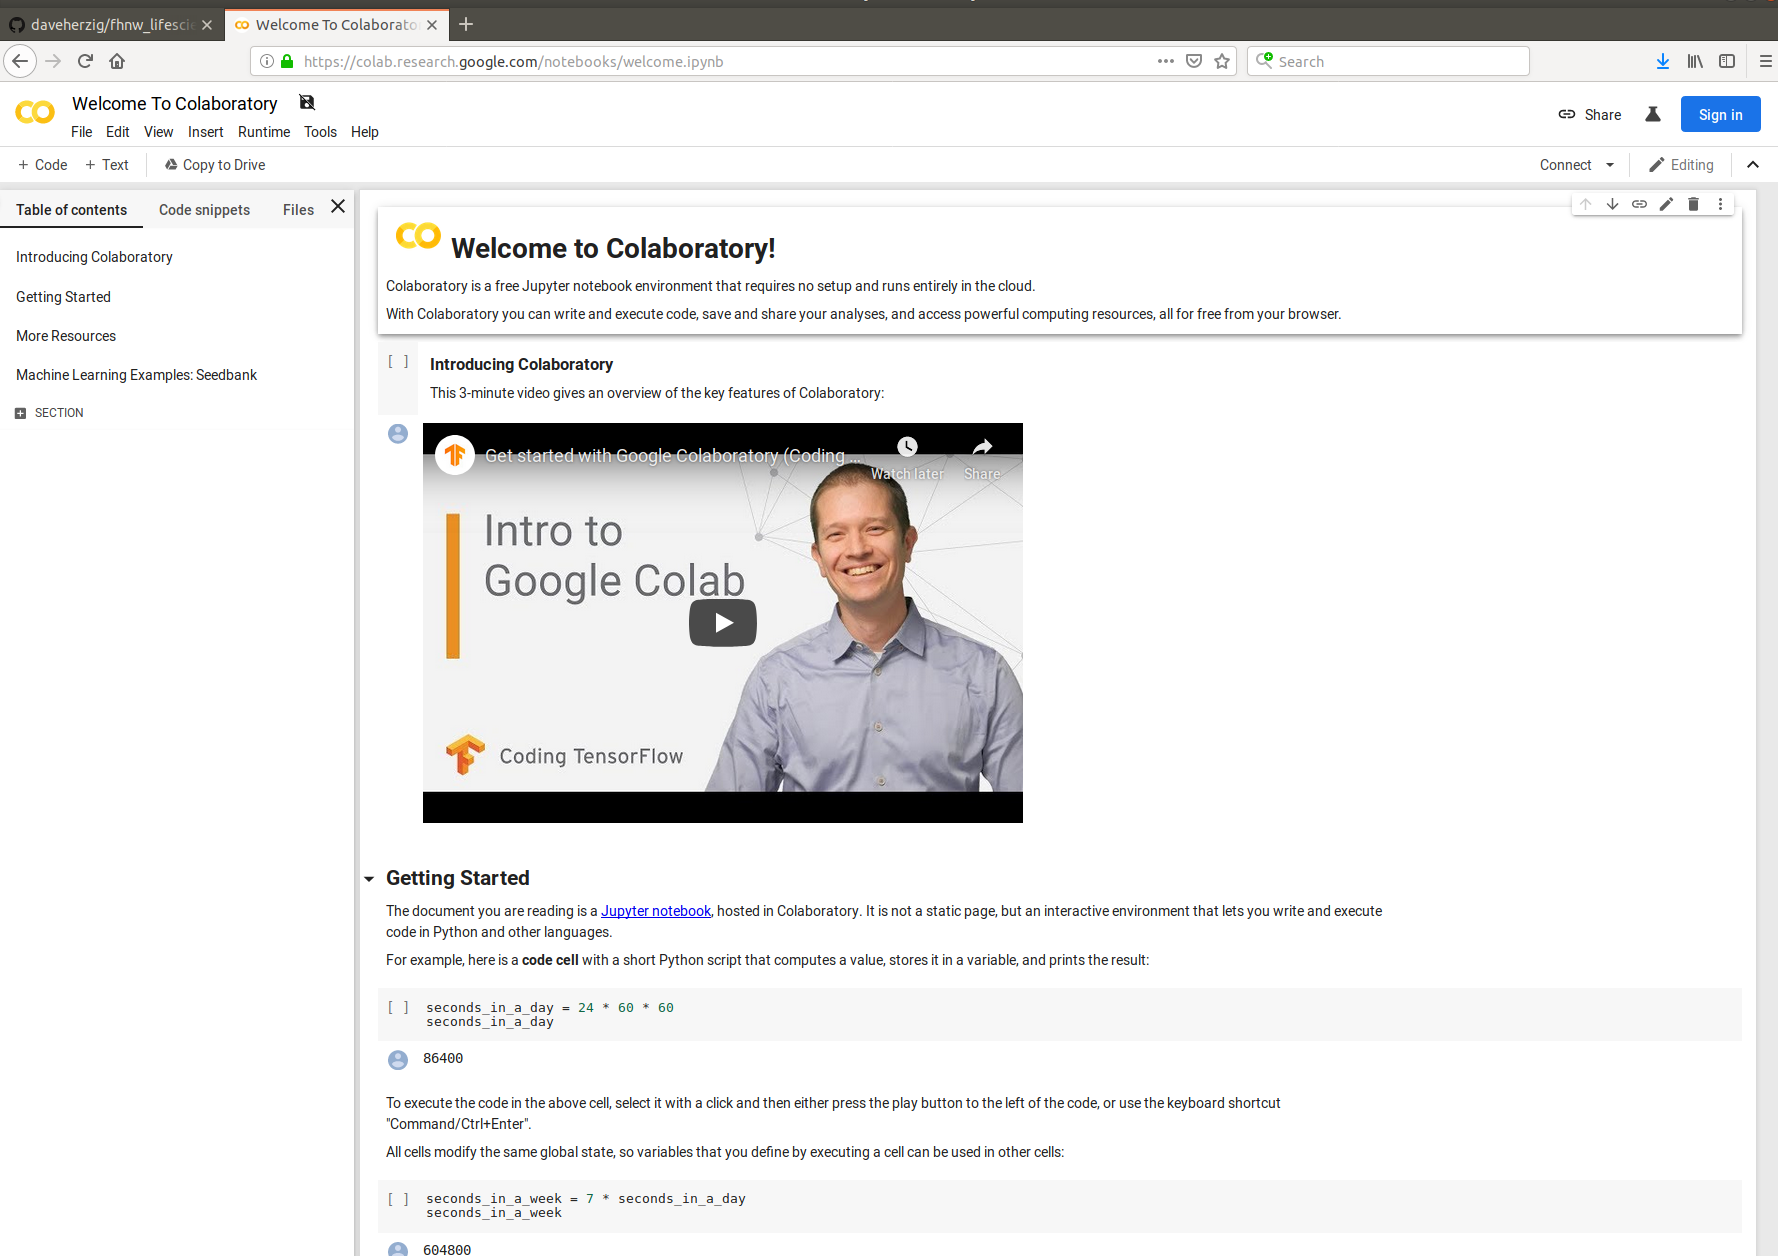
\includegraphics[scale=0.1]{img/jupyter_notebook}
\end{frame}


\begin{frame}[fragile]
  \frametitle{Python Frameworks}
  The following python frameworks will be used:
  \begin{itemize}
  \item Numpy
  \item Pandas
  \item Tensorflow
  \end{itemize}
\end{frame}

\begin{frame}[fragile]
  \frametitle{Jupyter Notebook}
  \begin{exercise}
  Write (and run) your first Jupyter notebook on Google Colab!
  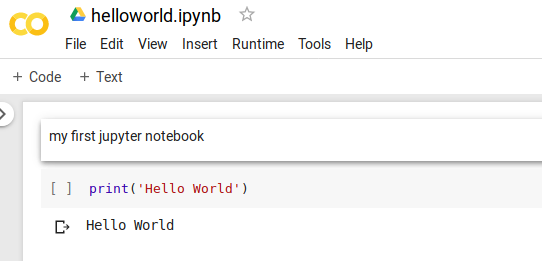
\includegraphics[scale=0.5]{img/jupyter_notebook_exercise}
  \end{exercise}
\end{frame}
